
\begin{frame}
\frametitle{Introduction - Model Driven Engineering}

	\begin{figure}
		\begin{minipage}[b]{0.38\textwidth}
			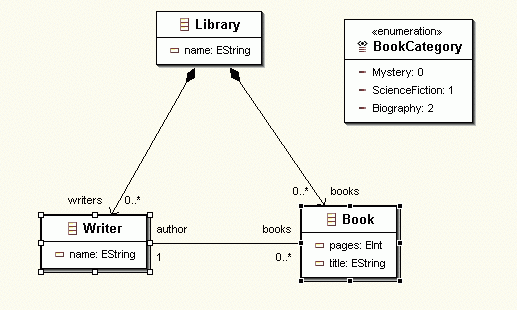
\includegraphics[width=0.9\linewidth]{figures/sample_model.png}
		\caption{A sample model [Eclipse, 2014]}
		\label{uml_sample}
		\end{minipage}
	\begin{minipage}[b]{0.4\textwidth}
		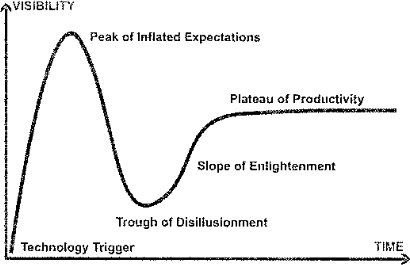
\includegraphics[width=0.9\linewidth]{figures/mde_pos.jpg}
	\caption{The technology hype cycle [M. Brambilla, 2012]}
	\label{mde_pos}
	\end{minipage}
	\begin{minipage}{0.1\textwidth}
	\vspace{10mm}
	\end{minipage}
	\end{figure}
\end{frame}


\begin{frame}
\frametitle{Introduction - Model Driven Engineering}

	\begin{figure}
	\centering
	
\includegraphics[scale=0.5]{./presentation/images/epsilon}
	\end{figure}
	
	\begin{itemize}
	\item Has a set of languages for MDE purposes
	\item Languages are interpreted
	\end{itemize}
\end{frame}

\begin{frame}
\frametitle{Motivation}
	\begin{figure}
		\centering
		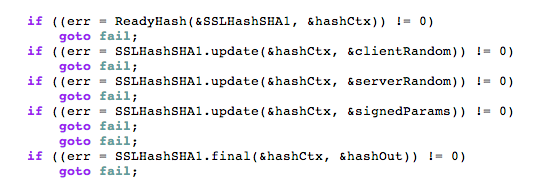
\includegraphics[width=0.758\linewidth]{figures/appleBug.png}
		\caption{Apple's SSL Bug [Imperial Violet, 2014]}
	\end{figure}
\end{frame}


\begin{frame}
\frametitle{Motivation}
\begin{itemize}
\item Epsilon currently lacks any test coverage metrics.
\item Useful features will attract more users to MDE, and improve the quality of MDE tools.
\end{itemize}
\end{frame}


\begin{frame}
\frametitle{Introduction - Software Testing Metrics}
	\begin{figure}
		\centering
		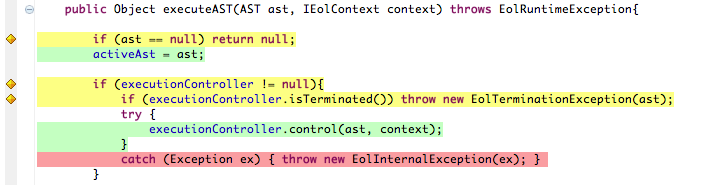
\includegraphics[width=0.758\linewidth]{figures/EclEmma}
		\caption{EclEmma [EclEmma.org, 2014]}
	\end{figure}
	\begin{itemize}
	\item Statement Coverage
	\item Branch Coverage
	\item Path Coverage
	\end{itemize}
\end{frame}

%\begin{frame}
%\frametitle{Introduction - Software Testing Metrics}
%\begin{figure}
%\centering
%\begin{minipage}{.3\textwidth}
%  \centering
%  \lstinputlisting[language=EOL]{code/statements/if.java}
%  %\caption{}
%  %\label{lst:blockStatement}
%\end{minipage}%
%\begin{minipage}{.3\textwidth}
%  \centering
%  \includedot[width=\linewidth]{figures/statements/if_AST}
%   % \caption{}
%  %\label{fig:blockAST}
%\end{minipage}
%\begin{minipage}{.3\textwidth}
%  \centering
%  \includedot[scale=0.3]{figures/statements/if_CFG}
%   % \caption{}
%  %\label{fig:blockCFG}
%\end{minipage}
%\caption{From left to right: Code for an if statement, its AST and its CFG}
%\end{figure}

%\end{frame}